\documentclass[12pt]{article}

\usepackage{hyperref}
\hypersetup{
	colorlinks,
	citecolor=blue,
	%filecolor=black,
	linkcolor=black,
	urlcolor=blue
}
\usepackage{float}
\usepackage[english]{babel}
\usepackage[square,numbers]{natbib}
\bibliographystyle{abbrvnat}
\usepackage{url}
\usepackage[utf8x]{inputenc}
\usepackage{amsmath}
\usepackage{graphicx}
\graphicspath{{images/}}
\usepackage{parskip}
\usepackage{fancyhdr}
\usepackage{vmargin}
\PassOptionsToPackage{hyphens}{url}\usepackage{hyperref}
\setmarginsrb{3 cm}{2.5 cm}{3 cm}{2.5 cm}{1 cm}{1.5 cm}{1 cm}{1.5 cm}
\usepackage[table]{xcolor}
\usepackage{todonotes}
\usepackage{menukeys}

\title{Spatiotemporal Data Classification}   % Title
\author{ Nikiforos Pittaras, M1422 \\ 
		 Chrysoula Themeli, M1423}                               % Authors
\date{\today}  % Date

\makeatletter
\let\thetitle\@title
\let\theauthor\@author
\let\thedate\@date
\makeatother

\pagestyle{fancy}
\fancyhf{}
%\rhead{\theauthor}
\lhead{\thetitle}
\cfoot{\thepage}

\begin{document}
	
	%%%%%%%%%%%%%%%%%%%%%%%%%%%%%%%%%%%%%%%%%%%%%%%%%%%%%%%%%%%%%%%%%%%%%%%%%%%%%%%%%%%%%%%%%
	
	\begin{titlepage}
		\centering
		\vspace*{0.5 cm}
		
\includegraphics[scale = 0.75]{ekpalogo.png}\\[1.0 cm]   % University Logo
		\textsc{\LARGE National and Kapodistrian University of Athens}\\[2.0 cm]   % University Name
		\textsc{\Large Department of Informatics and Telecommunications}\\[0.5 cm]               % Department
		\textsc{\large Large-Scale Data Analysis Techniques}\\[0.5 cm] % Course Name
		\rule{\linewidth}{0.2 mm} \\[0.4 cm]
		{ \huge \bfseries \thetitle}\\
		\rule{\linewidth}{0.2 mm} \\[1.5 cm]
		
		\begin{minipage}{0.4\textwidth}
			\begin{center} \large
				\theauthor
			\end{center}
		\end{minipage}~
		\begin{minipage}{0.4\textwidth}
		\end{minipage}\\[2 cm]
		
		{\large \thedate}\\[2 cm]
		
		\vfill
		
	\end{titlepage}
	
	%%%%%%%%%%%%%%%%%%%%%%%%%%%%%%%%%%%%%%%%%%%%%%%%%%%%%%%%%%%%%%%%%%%%%%%%%%%%%%%%%%%%%%%%%
	
	\tableofcontents
    \newpage
	\listoffigures
	\newpage
	\listoftodos
	\newpage
	
	%%%%%%%%%%%%%%%%%%%%%%%%%%%%%%%%%%%%%%%%%%%%%%%%%%%%%%%%%%%%%%%%%%%%%%%%%%%%%%%%%%%%%%%%%
	\section{Introduction}
    This is the report related to the Python project for the course "Large-Scale Data Analysis Techniques". In the below sections, the implemented logic will be explicitly analyzed. The project is divided in two parts: in the first part the goals are: to preprocess and clean the given data as well as to visualize five of the given trips in the train\_set file. In the second part, the tasks are: to find for all test trips the k nearest neabours from the given train trips, to find the train trips with the longest similar subroute for each test trip, to use 10-fold cross validation to the training data and classify them with three different methods (k-nearest neighbours, logistic regression and random forest) and finally to choose one of the above classification methods and improve the result.
    
    In the Main.py file, it is required to provide the path to the output folder as well as the input file with the training data. Afterwards, three folders are created to keep the images with the trips' visualizations for questions 1c, 2a1 and 2a2 and then the functions implementing the project's tasks are called.
    
	\section{Exercise 1}
	In this section, further details are provided related to the preprocessing and cleaning of the training data as well as to the trip's visualization. All files implementing the requirements of this part are in the folder FirstQuestion.
	
	\subsection{Question A}
	The first task of the project was to pre-process the given data, which is implemented in the file Preprocessing.py. In the read\_file\_contents, the train\_set.csv file is provided as input and for each line the necessary information is stored in a dictionary (journey\_id, vehicle\_id, timestamp, longitude and latitude).
	
	Since now the data from the input file are stored in the dictionary, the next step is to save the data based on the vehicle id. The function get\_data\_per\_vehicle\_id gets this dictionary as input and for every object in the dictionary, creates a list with key the vehicle\_id and then stores the remaining data connected with this id. The same process is followed for the sorting of data based on the journey\_id, therefore the structure where data are stored is a dictionary with key the vehicle\_id and with value another dictionary with key the journey\_id and with value a list containing several lists with the timestamp, the longitude and the latitude information.
	
	Finally, in the function get\_trips, the above structure is stored in the file trips.csv. The output format follows the requested pattern giving each trip an id. The final data structure is a list where each item has the trip\_id, the journey\_id and lists containing the timestamp, the longitude and the latitude.
	
	\subsection{Question B}
	The second goal was to clean the given data, based on the total trip distance and the max distance between two successive points. Total distance should not be less than 2km and max distance should not exceed 2km.
	
	The above logic is implemented in the file CleanData.py in function filter\_trips. The two lists (trips\_too\_small and trips\_too\_big) will keep the excluded trips due to either not valid total distance or to invalid max distance between successive points. For each trip in the list (returned from question A) the total distance is calculate, using the function calculate\_lonlat\_distance, which returns the distance between two successive points using the haversine formula. Following the same logic, the max distance between successive points of a trip is calculated and a distance is found more than 2km, the trip is excluded.
	
	Finally, the cleaned trips are kept in a list under the same format that was used in Question A and they are extracted in the file cleanTrips.csv, but also in the file tripsClean.pickle which keeps the data structure used. The functions for the data export are in the file utils.py (write\_trips\_to\_file and write\_trips\_using\_pickle).
	
	\subsection{Question C}
	This task is implemented in the file DataVisualization.py and the created output is stored in the folder Question1C. The requirement is to visualize five of the given train trips. For this purporse, a new trips list is creating containing five trips, excluding all trips with null journey\_id. Afterwards, the data\_visualization function is called, and a points list is created having two tuples with all the longitudes and latitudes(function idx\_to\_lonlat in the utils.py). 
	
	Finally, the function write\_group\_gml from the utils.py file is called. In this function, it is calculated the mean for both longitudes and latitudes and then gmplot is uded so as to visualize the selected trips. Below, there is an example of a trip shown on map is presented:
	
	\begin{figure} [H]
		\begin{center}
			
\includegraphics [scale = 0.75] {questionCexample.jpg}
			\caption{Example of trip visualization}
		\end{center}
	\end{figure} 
	
	\section{Exercise 2}
	The files implementing the requirements of this part are in the folder SecondQuestion.
	
	\subsection{Question A1}
	For this part a test file is given (test\_set\_a1.csv) containing additional trips. For each of these trips, the k nearest neighbours are targeted (in this exercise k=5) and an image file is produced, showing all six trips (the test trip and the trips from the training file) on six different maps. Under each map, the neighbour index, the journey\_id, the dynamic time warping and the time needed to process the neighbours of this test trip in millisec.
	
	The code for this question is in the file NearestNeighbours.py. Firstly, all test trips in the test file are extracted and stored in the same data structure as the trip list that contains the training dataset. Subsequently, for each test trip all nearest neighbours are calculated in the function find\_nearest\_neighbours\_for\_test\_trip, keeping the time needed in a variable. At the beginning of the trips processing, the tic method from utils.py file is used (finds the current time in millisec using the datetime.datetime.now() method). After having found the nearest neighbours for the given test trip, the method tictoc() is called, returning the required time. In order to find the nearest neighbours, the following process is implemented: For the test trip and all the training trips, the longitudes and latitudes are stored in tuples which are provided to the function calculate\_dynamic\_time\_warping in order to find the distance between two points. The calculated distances are stored in a list, which finally is sorted in ascending order and only the five nearest neighbours are kept.
	
	Since now the nearest neighbour trips are found, the trips list is updated (function: get\_updated\_trips\_list) containing now only those five trips. The final step now is to visualize the six trips. For this purpose, three list are created: a list with all the points (longitudes and latitudes), a list with the labels and a list with the colors (in this question the only color is the blue). All this data is provided to the function visualize\_paths in the utils.py file in order to export the trips as map images.
	
	In order to be able to create an image containing all the six maps each time, the rasterize.js file is required as well as phantomjs. In this function, both .html and .jpg files are created. First of all, the function write\_group\_gml is used so as to create the html files (this function is described above in question c). These html files are converted to images using the function html\_to\_png. File names are kept in a list and when the final image file is created (containing all six maps) these files are deleted. Afterwards, images as displayed as collection of plots and exported in the .jpg format.
	
	An example of this question image output can be found below:
	
	\begin{figure} [H]
		\begin{center}
			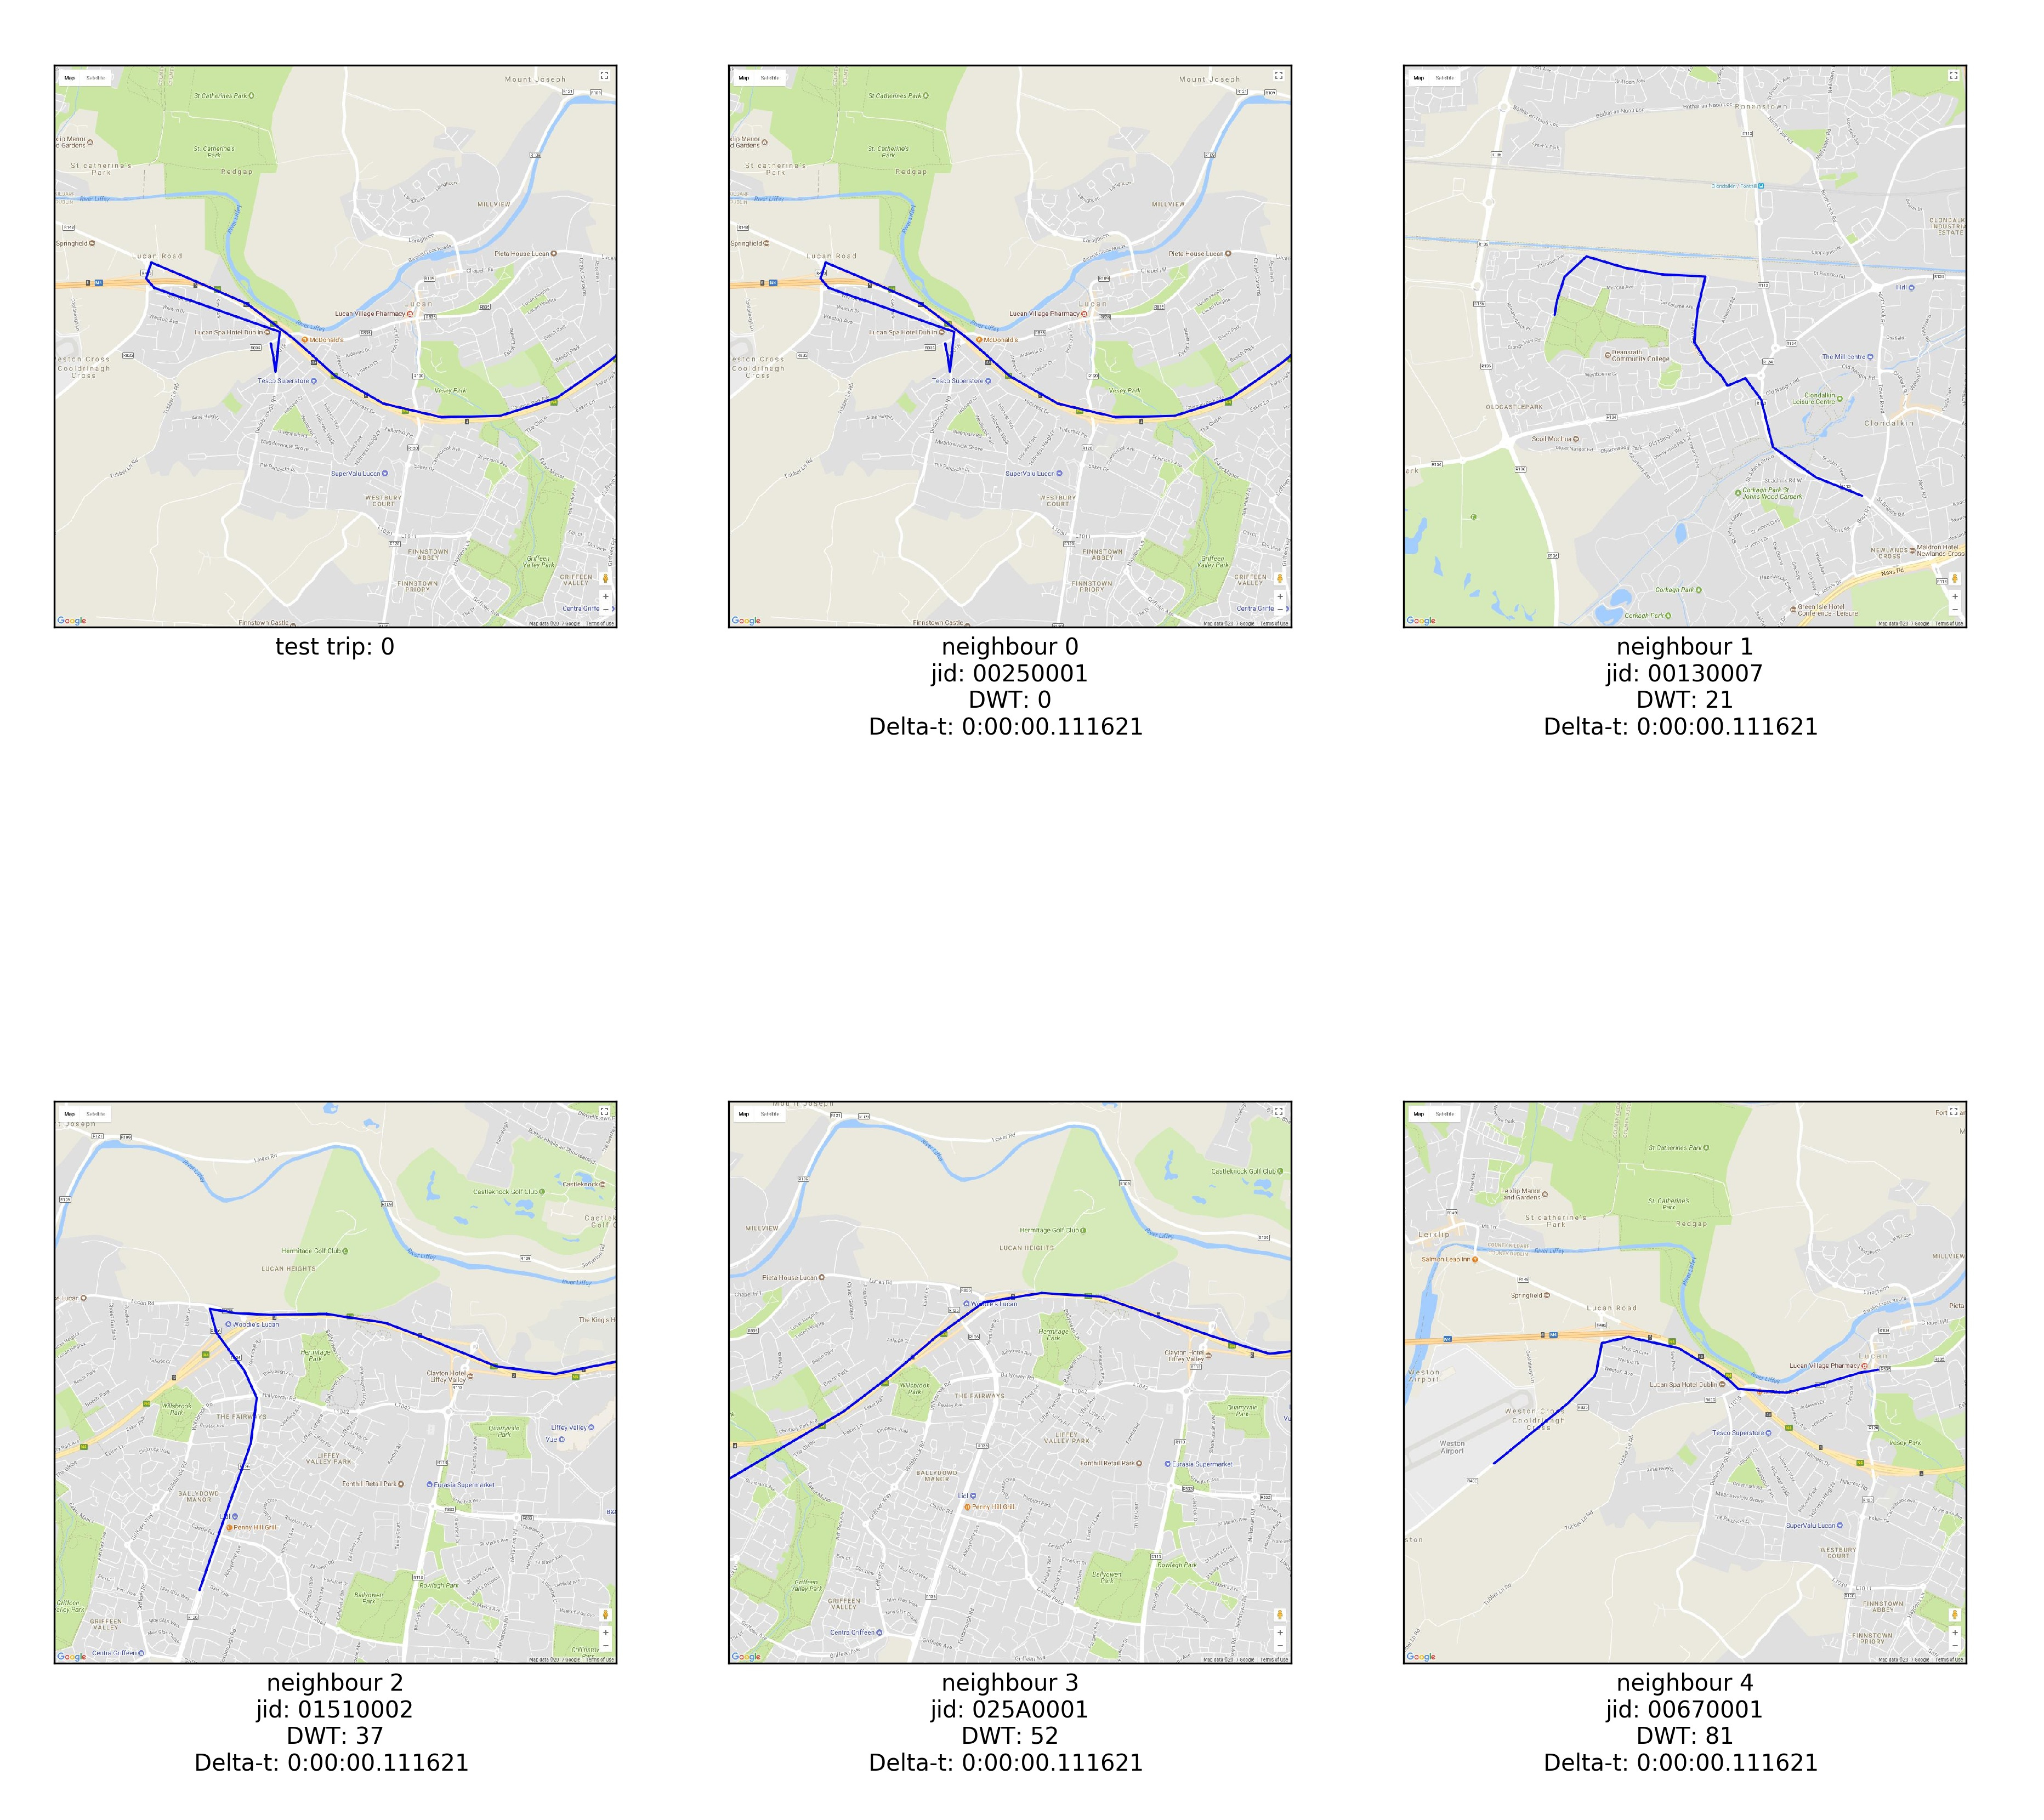
\includegraphics [scale = 0.50] {question2a1example.jpg}
			\caption{Example of nearest neighbours trips visualization}
		\end{center}
	\end{figure} 
	
	\subsection{Question A2}
	Following the same logic as above, the given test file(test\_set\_a2.csv) is parsed storing the data in the usual format and the function find\_similar\_subroots\_per\_test\_trip is used to determine the nearest sub-routes for each test trip.
	
	Similarly to the above question, the points are stored as tuples and the required time is calculated using the relevant methods from the utils.py file. To begin with, the method calc\_lcss is called
	\todo{describe calc and update lcss}
	
	Finally, a similar data preprocessing is followed before visualize the data. This time the points are separated so as to show which of them belong to the nearest subroute and color them with red color. The function for the visualization is the same that was used for the question 2A1.
	
	\subsection{Question B}
	The purpose of this task was to export features for classification for the training dataset. In short, a grid should be created and the points of each trip trace should be replaced by a specific square of the grid. The output file where the exported features are stored is the tripFeatures.csv and the tripFeatures.pickle, which was used in order to keep the final data structure with the features.
	
	In order to be able to draw the grid, it was necessary to find the min and max longitudes and latitudes (function: find\_min\_max\_latlong). Having now this information, the next function called is the create\_grid giving as input the number\_of\_cells and the result of the previous method. The distance per cell in the grid is calculated as the difference between the max and the min lat/long divided by the total number of cells. The next step is to create the lines of the rows and the columns and then to provide a name for each cell.
	\todo{explain the replacepoints}
	
	Finally, the method visualize\_grid is called.
	\todo{explain the function}
	
	\subsection{Question C}
	
	
	\subsubsection{Beat ​ ​the ​ ​Benchmark}
	
	\newpage
	\addcontentsline{toc}{section}{References}
	\begin{thebibliography}{30}
		\bibitem{first} 
    \end{thebibliography}
	
\end{document}